\chapter{Analysis}
\label{chap:analysis}

Knowledge of the positions of robots and knowledge of the environment is essential for solving complex tasks efficiently in multirobot systems. Over time various techniques evolved to acquire this knowledge.

\section{Map-merging}

This work focuses on multirobot systems consisting of mobile robots, each capable of building a \gls{3D} map of the surrounding environment. Typically each robot uses a \gls{SLAM} algorithm to create a map and is equipped with appropriate sensors such as stereo camera rigs, active \gls{RGB-D} cameras or laser range finders. Such sensors are available in the broad weight and cost range enabling large variety of \gls{SLAM}-capable robots operating both on the ground and in the air. This variety leads to possible heterogeneous teams of robots capable of solving broad range of tasks.

The \textit{map-merging problem} for multirobot systems, which is the focus of this work, is to estimate positions of the robots in the environment and to merge the maps from individual robots to produce a single globally consistent map.

\section{The map representation}

\Gls{3D} maps are becoming more common in the robotics as the capable sensors are getting more affordable and suitable for many applications. Unlike \gls{2D} occupancy grids used extensively in the past, \gls{3D} maps enable cooperation of robots, that are not fixed to a \gls{2D} plane, such as aerial vehicles, humanoid robots, outdoor robots operating in a rough terrain as well as traditional ground-based platforms. This allows us to create a possibly heterogeneous multirobot teams, that are able to take advantage of their different strengths and weaknesses to solve the assigned task efficiently. For example a robotic team can consist from aerial vehicles, capable of fast reconnaissance in large-scale outdoor environments, and ground-based vehicles carrying heavy equipment.

This work expects maps represented as pointclouds (definition~\ref{def:pointcloud}). Pointclouds can be implemented as an array of points, making them suitable for serialisation and exchange between robots. Points in the pointcloud can have assigned additional information, such as \gls{RGB} colour information or reflection intensity, based on the available sensor. Especially colour information, that is provided by stereo camera rigs and active \gls{RGB-D} cameras is commonly exploited for further processing (figure~\ref{fig:v1-greyscale}).

\begin{figure}
    \centering
    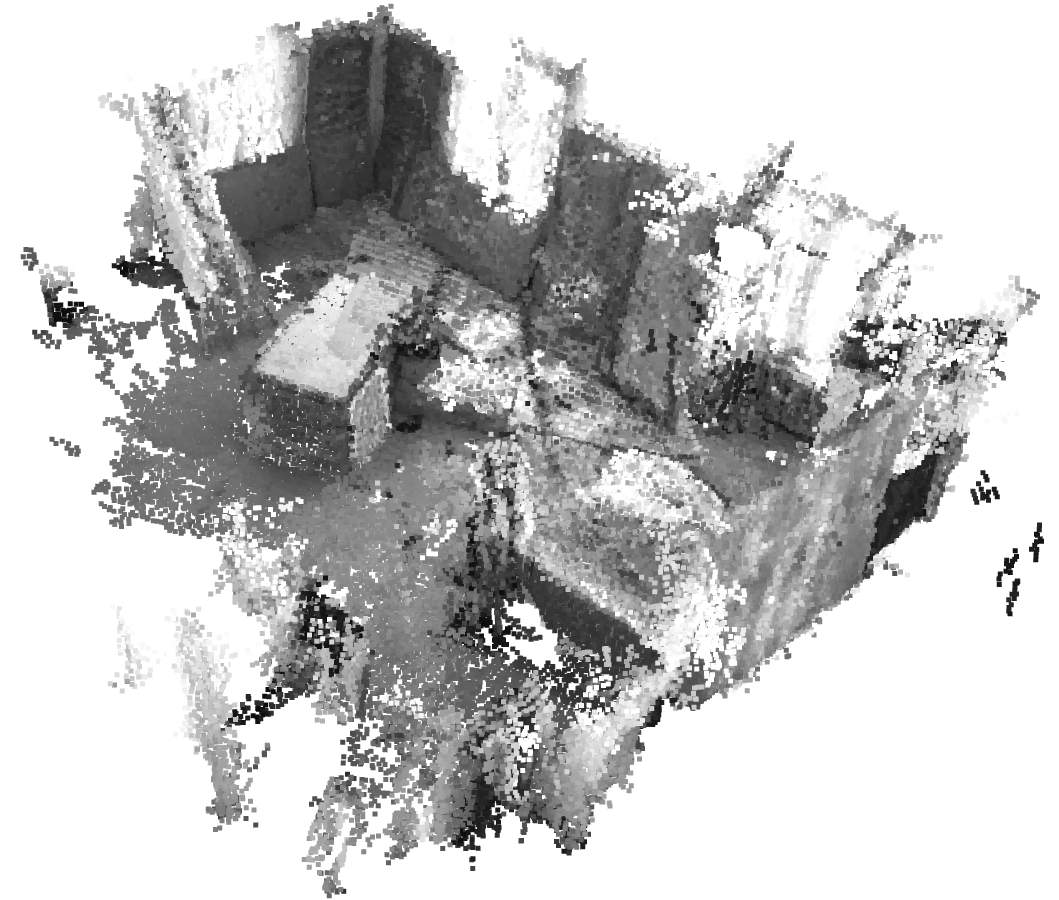
\includegraphics[width=\textwidth]{../img/v1-greyscale.png}
    \caption[Pointcloud map with greyscale colours]{Partial pointcloud map of a room created from aerial vehicle equipped with greyscale stereo cameras rig. Intensity captured by camera is stored alongside the points and visualised in greyscale.}
    \label{fig:v1-greyscale}
\end{figure}

\begin{defn}[Pointcloud]
\label{def:pointcloud}
A pointcloud is a set of data points in space.
\end{defn}

Other datastructures used in the \gls{3D} mapping, such as octree-based maps used by~\citet{hornung2013octomap}, can be converted to pointclouds without any loss of information, because pointclouds do not pose any restrictions on the geometry of the points and it is easy to add metadata associated with the points. This makes pointclouds suitable datastructure for exchange between different mapping approaches, even when they use different representations internally.

Pointclouds data messages are supported and well established in the \gls{ROS} framework. There are mature libraries to work with pointclouds, such as \gls{PCL}. This makes pointclouds suitable map representation for multi-robot systems.

\section{Direct map-merging}

Early map-merging techniques, classified as \textit{direct map-merging} by~\citet{lee2012survey}, use direct sensor measurements to compute the transformation between robots. This involves especially the case of robot rendezvous used by~\citet{zhou2006rendezvous}, which relies on robots' ability to sense each other position directly. Popular technique uses camera and special recognizable markers on the robots to compute the transformation using computer vision algorithms.

A robot rendezvous might be hard to achieve in large-scale environments, especially if the robots are starting from different locations or in a different time (for example to react to increasing demands for the service). Such applications typically need map-merging to be able to work only with sensed surrounding environment instead of the presence of other robots in the same space.

Direct map-merging also involves techniques relying on global localization in the environment being available. This involves a purpose-adapted environments with installed markers or beacons to locate robots within environment and systems using global localization such as \gls{GPS}.

While purpose-adapted environments may greatly simplify map-merging problem, they make deployment of the multirobot systems harder and might introduce severe costs. For applications such as space exploration, disaster rescue, victim search and mine cleaning any modifications of the environment are not conceivable and in many more applications such as unmanned delivery the modifications are usually not practical.

Global localization systems are usually not available indoor and while such systems are a great aid for navigating large-scale outdoor environments, the provided accuracy is usually not high enough for merging high resolution pointcloud maps. The position from global localization systems can be however used as an initial guess for map-merging algorithms.

\section{Map-merging on occupancy grids}

Later developed techniques work with \gls{2D} maps, usually represented as occupancy grids. \citet{lee2012survey}~categorize this techniques as \textit{indirect map-merging}. These techniques rely on overlapping areas in maps for map-merging.

Using \gls{2D} maps limits operational space of robots and practically limits multirobot teams to only ground-based vehicles operating indoor or in light terrain, flat environments. Particularly \gls{2D} maps prohibits promising multirobot teams consisting of aerial and ground-based vehicles.

Map-merging techniques for \gls{2D} occupancy grids involves spectra-based approach of~\citet{carpin2008spectra} and image feature-based approach of~\citet{Horner2016}. The latter algorithm is available in the \gls{ROS} distribution as ready-made solution for merging \gls{2D} maps.

\section{Map-merging as distributed SLAM}

Map-merging algorithms have been also implemented as distributed \gls{SLAM} algorithms. These techniques take advantage of the research in the area of \gls{SLAM} algorithms and use loop-closure techniques developed for \gls{SLAM} to implement map-merging. Especially graph-based \gls{SLAM} implementations can be naturally extended to merge maps from multiple robots. Nodes from other robots can be added to the \gls{SLAM} graph and connected through loop-closures with existing nodes to form a single map.

When a loop-closure between 2 maps is detected, it can be used to compute the transformation between maps. We need to extend the loop detection to work across map boundaries, not only within a single map as usual in the \gls{SLAM}, which typically requires exchanging implementation-specific data between robots. This poses several disadvantages. Based on the \gls{SLAM} loop-closure approach the internal \gls{SLAM} data may be quite large (see table~\ref{tabl:rtabmap-db-vs-pointclouds}), stressing communication bandwidth. Exchanging implementation-specific data usually leads to running the same \gls{SLAM} algorithm on all robots in the multirobot system, or the implementations must be adapted to exchange compatible loop-closure data. This is challenging for heterogeneous multirobot systems, when individual robots use different sensors, which is often the case when using both ground-based and aerial robots. For example if ground-based robots are equipped with accurate heavy \gls{3D} laser range finder and aerial vehicles use lightweight stereo rig cameras, the \gls{SLAM} approaches are typically different and the loop-closure data are inherently incompatible (image features and \gls{3D} laser scans). In such scenarios we need to use a different approach.

\citet{lee2012survey}~list scan matching loop closure approaches used for map-merging, which are used with \gls{2D} \gls{SLAM} algorithms. \gls{2D} distributed \gls{SLAM} based on scan matching was implemented by~\citet{pfingsthorn2007scalable} for RoboCup Rescue Virtual Robots competition. \citet{fox2006distributed} used a direct exchange of laser range scans and odometry motion information coupled with a particle filter to localize robot in the second map.

In \gls{3D} camera-based \gls{SLAM} algorithms, visual appearance-based techniques are particularly popular. \citet{tomono2013merging} used appearance-based algorithm based on \gls{SIFT} features to merge visual maps, validated by travelled paths to reject false similarities in repetitive environments. Visual bag-of-words loop closure approach was used by~\citet{labbe2014online} to merge maps in multi-session \gls{SLAM}. Multi-session \gls{SLAM} works with maps generated by a single robot starting consecutively in the different positions. In such setup there is no need for communication, so a local database was used by the authors to store loop-closure related data for map-merging.

\section{Map-merging on pointclouds}

The algorithm presented in chapter~\ref{chap:mergingalgorithm} works exclusively with \gls{3D} pointclouds without any additional exchange of data to offer maximum flexibility. The algorithm does not require any exchange of implementation-specific data and can be used with any \gls{SLAM} approach available, allowing future integration of the newest state-of-the-art methods in fast-paced \gls{SLAM} research. With the presented approach, each robot in the heterogeneous multirobot system can use a different \gls{SLAM} implementation, which allows using best-suited implementation to robot sensors and computational capabilities.

Using pointclouds can also save communication bandwidth especially compared to image-based loop closure methods, which may require to exchange significant amount of data. Size comparison between local database size used for map-merging by~\citet{labbe2014online}, implemented in popular \texttt{RTAB-Map} \gls{SLAM}, and pointcloud representation of the same maps is shown in table~\ref{tabl:rtabmap-db-vs-pointclouds}. The maps have been recorded at Charles University campus, see section~\ref{sec:mff-dataset} for details. The pointclouds are significantly smaller with resolution $0.05$ meter per voxel. The presented merging algorithm can work with resolution of just $0.1$ meter per voxel in which pointclouds are even smaller, so we could save more bandwidth if necessary.

\begin{table}[b!]
	\label{tabl:rtabmap-db-vs-pointclouds}
	\centering
	\begin{tabular}{lrr D{.}{.}{3}}
	\toprule
	\textbf{Map} & \textbf{Database} & \textbf{Pointcloud} & \textbf{Ratio} \\
	\midrule
	mff-mapping\_2018-04-06-13-43-39 & 217 MiB & 14 MiB & 0.066 \\
	mff-mapping\_2018-04-12-10-17-25 & 551 MiB & 33 MiB & 0.060 \\
	mff-mapping\_2018-04-12-11-04-51 & 231 MiB & 11 MiB & 0.048 \\
	mff-mapping\_2018-04-12-13-30-41 & 350 MiB & 16 MiB & 0.046 \\
	\bottomrule
	\end{tabular}
	\caption{Table comparing sizes of the local database of loop closure data for map-merging used by~\citet{labbe2014online} and the pointcloud representation of the same maps. Ratio denotes fraction of the pointcloud size to the database size. The maps are presented in section~\ref{sec:mff-dataset}.}
\end{table}

Note that the local database has been used only in multi-session \gls{SLAM} and might not be size-optimised. Still the table demonstrates order of magnitude differences between the two representations.

There are some challenges for map-merging on pointclouds. When using \gls{SLAM}-based approaches for map-merging, the resulting graph is usually optimized, which can repair mapping errors present in the individual maps. Repairing mapping errors in pointclouds maps is much harder. \citet{bonanni2017pose} addressed this problem by using pose graphs of pointclouds. In the pose graph representation the map is represented as a graph of smaller pointcloud sub-maps, not as one big pointcloud. This representation allows to repair maps in the similar manner as done in distributed \gls{SLAM} approaches, by optimizing the graph after merging.

Another challenge is to register the pointclouds (compute transformation between pointclouds) using only information stored within pointclouds. Algorithm implemented by~\citet{bonanni2017pose} relies on an external place recognition routine that reports matching pairs of local maps. The external routine is needed because authors used a pairwise registration algorithm, that needs an initialisation with a roughly-correct transformation to align pointclouds. The algorithm presented in chapter~\ref{chap:mergingalgorithm} can register pointclouds directly using a global registration approach that does not need any external place recognition routine. To the best of my knowledge, this approach is the first map-merging method
that can work directly on \gls{3D} pointclouds without any external pre-alignment routine.

Most of the methods for pointcloud registration are based on the \gls{ICP} algorithm introduced by~\citet{besl1992icp}. The \gls{ICP} algorithm uses an initial transformation estimate and it iteratively tries to minimise error metric (usually an euclidean distance between pointclouds). The initialisation is extremely important as the algorithm always finds a local minimum. Since the introduction of the \gls{ICP} algorithm, variants, reviewed in~\citet{pomerleau2015reviewregistration}, of the original algorithm has been developed, which are less susceptible to an accurate initialisation, but all \gls{ICP}-derived algorithms need the initialisation and are susceptible to local minima problems.

When using \gls{ICP}-family algorithms for scan matching in the context of \gls{SLAM}, the initial estimate is usually provided by the odometry source. In the map-merging problem the initial estimate must be provided from an external source, either manually by the operator or using an automated routine (for example vision-based place recognition method). The need for an accurate initial estimate is a severe drawback in the context of map-merging.

To be able to work without any initial estimate the algorithm presented in chapter~\ref{chap:mergingalgorithm} uses a feature matching approach, that does not require any initial estimate and is not affected by the initial configuration of the maps. These feature-matching approaches use descriptors developed specifically for pointclouds, such as \gls{PFH}, introduced by~\citet{rusu2008pfh}, to match keypoints between two maps. These algorithms has been developed for high-density pointclouds produced directly by sensors such as laser range finder and \gls{RGB-D} cameras. Some of the proposed features, such as \gls{NARF} introduced by~\citet{steder2010narf}, use range image representation and a single view-point assumption, that can not be generalised to \gls{3D} pointcloud maps. I show that it is viable to use feature-matching also for registration of low-density pointcloud when we take specifics of the pointcloud maps into account.
